\iffalse
\documentclass[12pt]{article}
\usepackage{amsmath}
\usepackage{graphicx}

\title{Gate 2023\_ec\_58}
\author{Hiba Muhammed \\
        EE23BTECH11026}

\begin{document}

\maketitle

\section*{Problem Statement}

Let $x_1(t) = u(t + 1.5) - u(t - 1.5)$ and $x_2(t)$ is shown in the figure below. For $y(t) = x_1(t) * x_2(t)$, the $\int_{-\infty}^{\infty} y(t) \, dt$ is \underline{\hspace{2cm}}.

\begin{figure}[htbp]
    \centering
    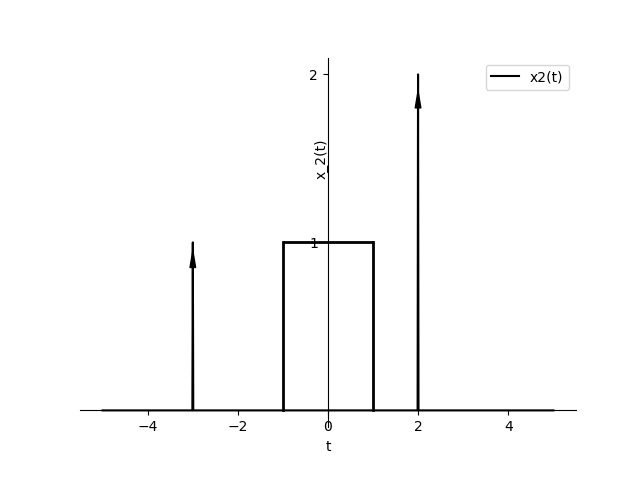
\includegraphics[width=0.5\textwidth]{2023/EC/58/figs/gatefig.png}
    \caption{Figure}
    \label{fig:graph}
\end{figure}

%\end{document}
